\documentclass[12pt]{article}

\usepackage{amsmath, color}
\usepackage{mdwmath}
\usepackage{amssymb, epsf, epsfig, textcomp}
\renewcommand{\baselinestretch}{1.3}
\usepackage{a4wide}
\newcommand{\argmin}{\mathop{\mathrm{argmin}}}
\usepackage{caption}
\usepackage{subcaption}
\usepackage{mathtools}
\usepackage{listings}
\lstdefinestyle{myCustomMatlabStyle}{
	basicstyle=\ttfamily\footnotesize,
	breaklines=true,
	language=Matlab,
	numbers=left,
	stepnumber=1,
	numbersep=10pt,
	tabsize=4,
	showspaces=false,
	showstringspaces=false
}
\begin{document}
	\noindent\rule{\textwidth}{2pt}
	\begin{center}
		{\bf Technical University of Crete}\\
		{\bf School of Electrical and Computer Engineering} \\
		Course: {\bf Wireless Communications 2022-2023} \\
		Exercise 2 (120/1000) \\
		Report Delivery Date: 24 November 2022 \\
		Instructor: Athanasios P. Liavas \\
	\end{center}
	{\bf Student: }Alevrakis Dimitrios 2017030001\\
	\rule{\textwidth}{.5pt}
	\vskip .1cm
	\noindent
	
	\begin{enumerate}
		\item[\bf Part 1]
		\begin{enumerate}
			\item[\bf 1]
			The block fading channels are created as described below:
			\begin{lstlisting}[language=octave]
h = zeros(M,N);
for div = 1 : M
	h(div,:) = (randn(1,N) + 1i*randn(1,N))*sqrt(1/2);
end
			\end{lstlisting}
			Where $M$ the desired diversity, meaning the number of receive antennae.
			
			\item[\bf 2]
			The transmitted 4-QAM symbols are created as described below:
			\begin{lstlisting}[language=octave]
s = 1 - (randi(2,[1,N])-1)*2 + 1i*(  1 - (randi(2,[1,N])-1)*2 );
			\end{lstlisting}
		
			\item[\bf 3]
			The White Gaussian noise is created as described below:
			\begin{lstlisting}[language=octave]
n = zeros(M,N);
for div = 1:M
	n(div,:) = ( randn(1,N) + 1i*randn(1,N) )*sqrt(N_0/2);
end
			\end{lstlisting}
			
			Therefore the received signal on each antenna is:
			\begin{lstlisting}[language=octave]
r = zeros(M,N);
for div = 1:M
	r(div,:) = h(div,:).*s + n(div,:);
end
			\end{lstlisting}
		
			The transmitted signal power:
			\begin{align*}
				P_{TX} = \mathcal{E}[s^2] = \frac{1}{N}\sum_{i=1}^{N}|s_i|^2 = \frac{1}{N}\sum_{i=1}^{N}|\pm1 \pm i|^2 = \frac{1}{N}\sum_{i=1}^{N}2 = 2
			\end{align*}
			Therefore the SNR in this case:
			\begin{align*}
				SNR_{db}=10log_{10}\frac{P_{TX}}{P_{noise}}=10log_{10}\frac{2}{N_0}
			\end{align*}
		
			In order to get the desired SNR:
			\begin{align*}
				N_0 = \frac{2}{10^{\frac{SNR_{db}}{10}}}
			\end{align*}
		
			\item[\bf 4]
			Using the Maximum Ratio Combining(MRC) method we define:
			\begin{align*}
				R\coloneqq\frac{{\bf h}^H}{||{\bf h||}}{\bf Y}
			\end{align*}
			and decide using the Maximum Likelihood(ML) method
			\begin{align*}
				{\bf x}^* = \underset{{\bf X}}{min}||{\bf R}-{\bf X}||^2
			\end{align*}
		
			\newpage
			\item[\bf 5]
			\begin{figure}[h!]
				\centering
				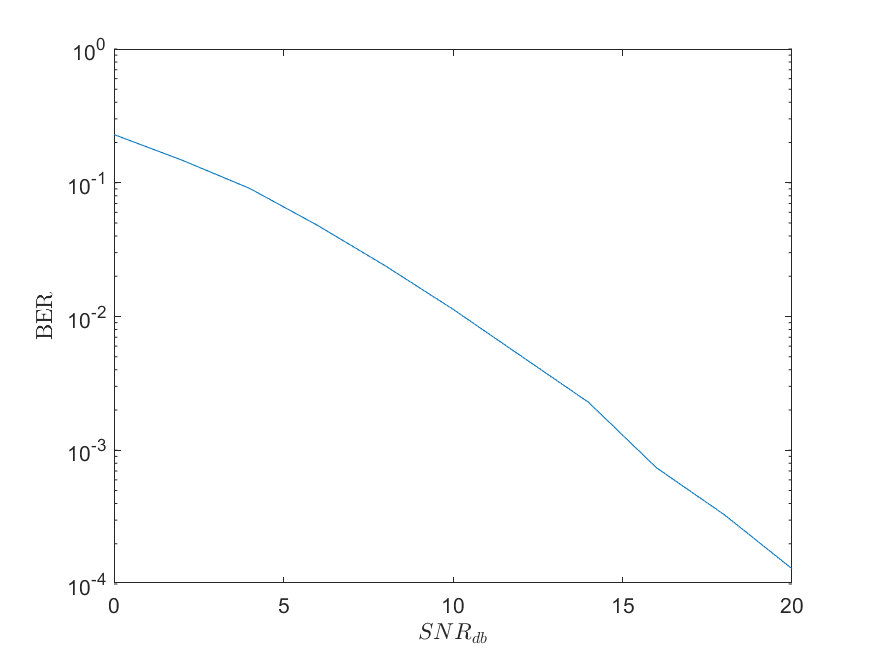
\includegraphics[width=0.5\textwidth]{fig1.png}
				\caption{MRC method: BER for $SNR_{db}=[0:2:20]$}
			\end{figure}
			
			
			\item[\bf 6]
			The theoretical BER:
			\begin{align*}
				BER_{Theoretical}=\begin{pmatrix}
					2M-1 \\ M
				\end{pmatrix}\frac{1}{4^MSNR_{db}^M}
			\end{align*}
			\begin{figure}[h!]
				\centering
				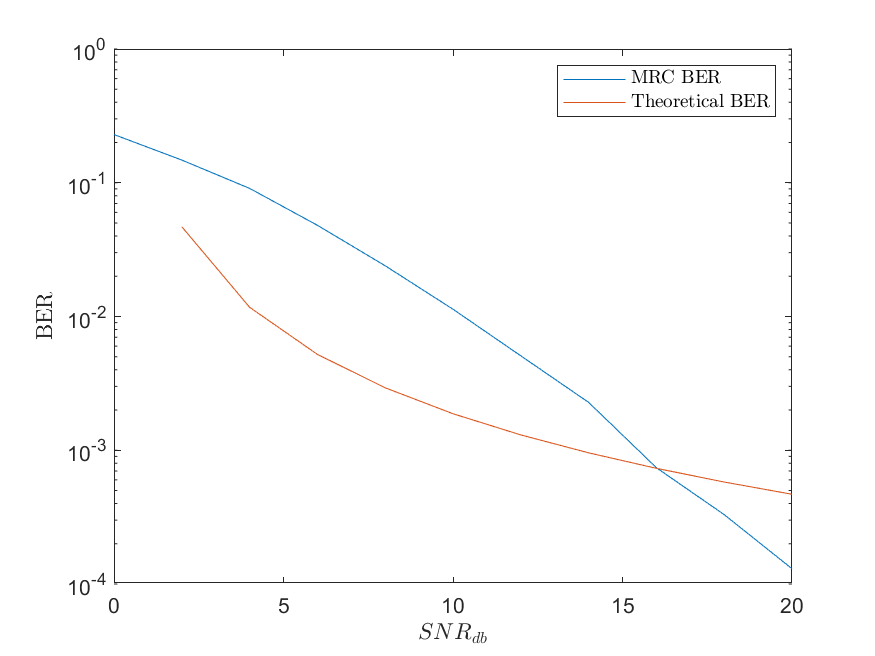
\includegraphics[width=0.5\textwidth]{fig2.png}
				\caption{MRC method: Experimental and Theoretical BER for $SNR_{db}=[0:2:20]$}
			\end{figure}
		
			As observed the Theoretical BER estimation, underestimates the experimental one for low SNR values but overestimates it for high SNR values.
			
			\newpage
			\item[\bf 7]
			\begin{itemize}
				\item Step 1 the same as before because since there are two transmit and one receive antennae, we have two channels to take into account.
				\item Step 2 the packets are created with the same method.
				\item In the Transmit Beamforming method the received signal is considered to be:
				\begin{align*}
					Y = ||{\bf h}||X + W
				\end{align*}
				
				Since we have one receive antenna and therefore one receive signal:
				\begin{lstlisting}[language=octave]
r = zeros(1,N);
for i = 1:N
	r(i) = norm(h(:,i),2)*s(i)+n(i);
end
				\end{lstlisting}
			
				\item Using ML we decide the received signal:
				\begin{align*}
					{\bf x}^* = \underset{{\bf X}}{min}||Y-{\bf X}||^2
				\end{align*}
				
				\item 
				\begin{figure}[h!]
					\centering
					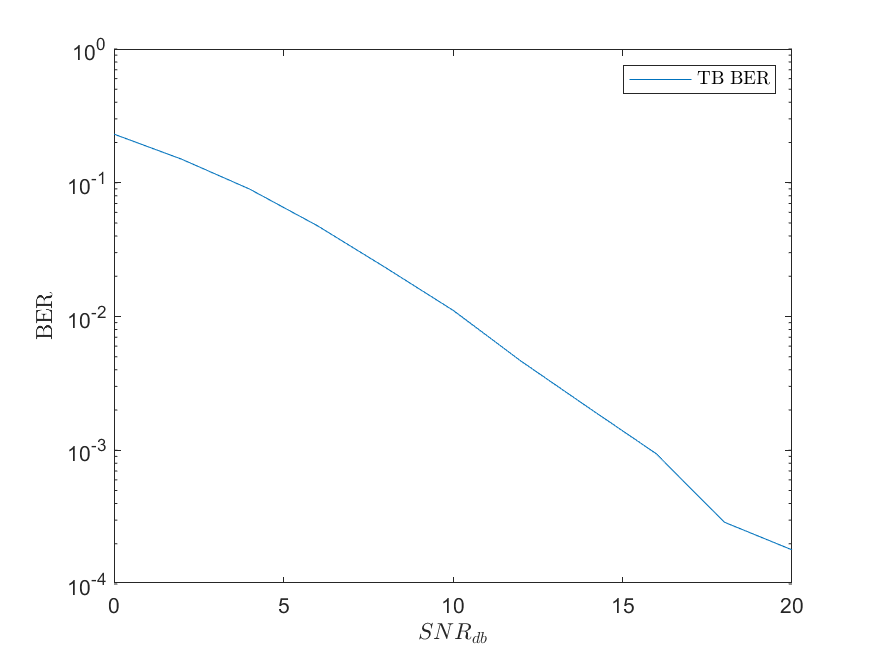
\includegraphics[width=0.5\textwidth]{fig3.png}
					\caption{TB method: BER for $SNR_{db}=[0:2:20]$}
				\end{figure}
			\end{itemize}
			\newpage
			\item[\bf 8]
			\begin{figure}[h!]
				\centering
				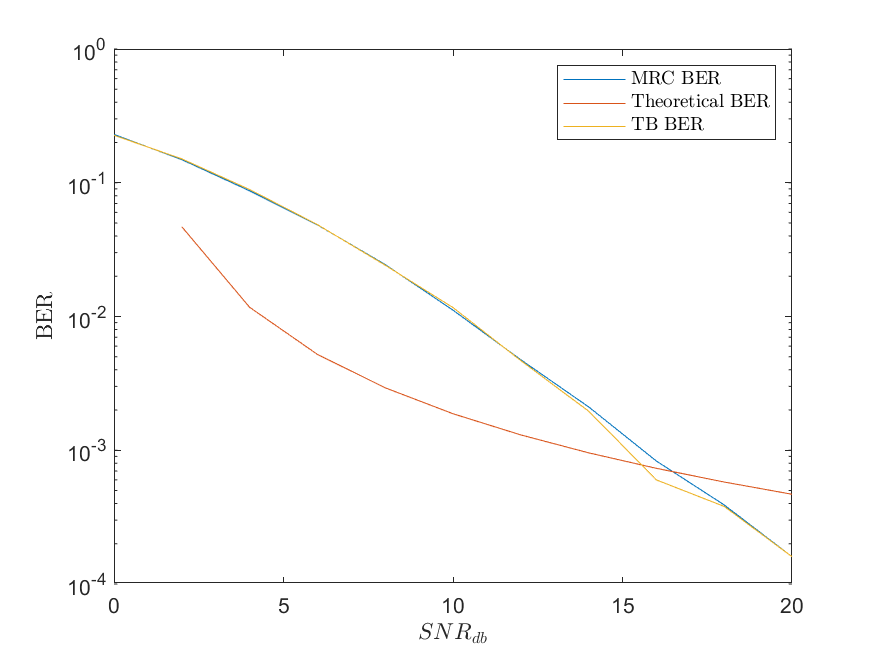
\includegraphics[width=0.5\textwidth]{fig4.png}
				\caption{MRC-TB-Theoretical: BER for $SNR_{db}=[0:2:20]$}
			\end{figure}
			The to methods (MRC and TB) have identical performance. This is on account of the fact that the transmitted signal on the TB method is constructed in order to receive the same signal as received on the MRC method($Y=||h||X+W$).
			
			\item[\bf 9]
			\begin{itemize}
				\item Step 1, In this case also, there are two channels because of the two transmitters and one receiver.
				\item Step 2 the packets are created with the same method.
				\item The received signal is:
				\begin{align*}
					\begin{bmatrix}
						Y_1 \\ Y_2^*
					\end{bmatrix}=
					\begin{bmatrix}
						h_1 & h_2\\ h_2^* & -h_1^*
					\end{bmatrix}
					\begin{bmatrix}
						X_1 \\ X_2
					\end{bmatrix}
					+ \begin{bmatrix}
						W_1 \\ W_2^*
					\end{bmatrix}
				\end{align*}
			
				\item We calculate:
				\begin{align*}
					\begin{bmatrix}
						R_1 \\ R_2
					\end{bmatrix}=\mathcal{H}^H
					\begin{bmatrix}
						Y_1 \\ Y_2^*
					\end{bmatrix}
				\end{align*}
				Where:
				\begin{align*}
					\mathcal{H}\eqqcolon\frac{1}{||{\bf h}||}\begin{bmatrix}
						h_1 & h_2 \\ h_2^* & -h_1^*
					\end{bmatrix}
				\end{align*}
				Then we decide: $\displaystyle x_1^* = \underset{{\bf X}}{min}||R_1-||{\bf h}||X||^2$ and $x_2^* = \underset{{\bf X}}{min}||R_2-||{\bf h}||X||^2$
				
				\newpage
				\item 
				\begin{figure}[h!]
					\centering
					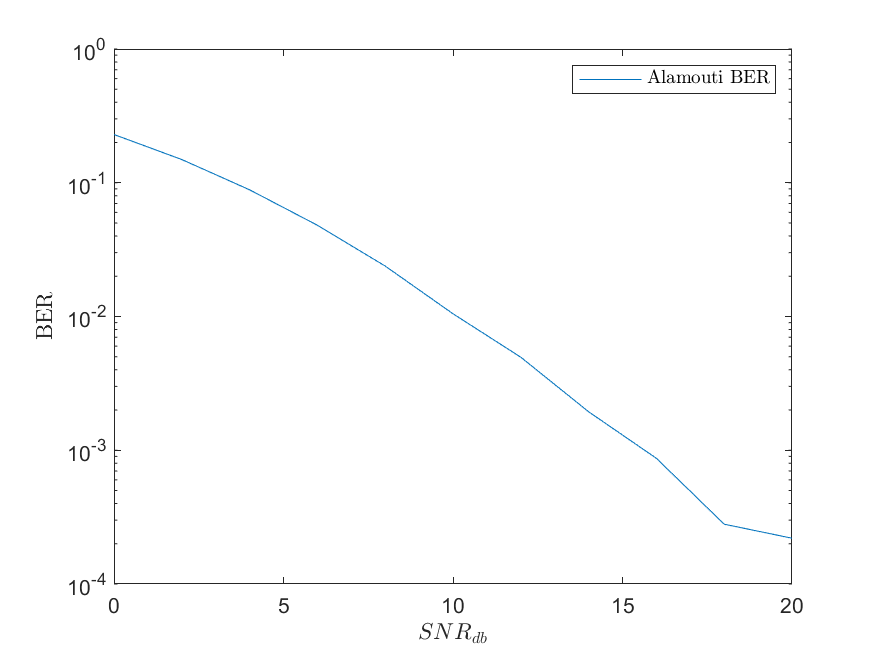
\includegraphics[width=0.5\textwidth]{fig5.png}
					\caption{Alamouti: BER for $SNR_{db}=[0:2:20]$}
				\end{figure}
			\end{itemize}
		
			\item[\bf 10]
			\begin{figure}[h!]
				\centering
				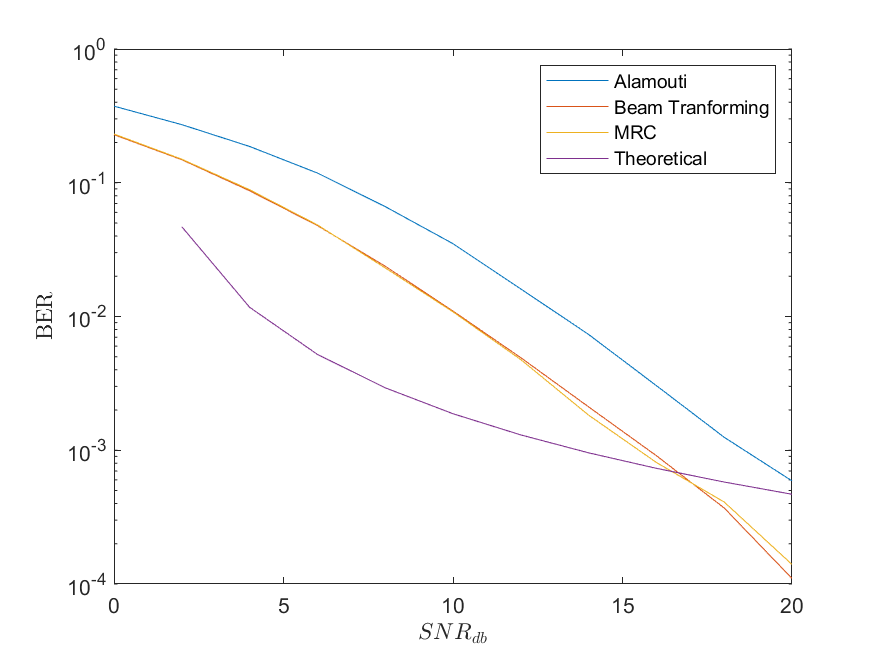
\includegraphics[width=0.5\textwidth]{fig6.png}
				\caption{Alamouti-MRC-TB-Theoretical: BER for $SNR_{db}=[0:2:20]$}
			\end{figure}
			Using the Alamouti method, two symbols are transmitted at the same time and therefore this method lack by 3 db from the other methods. For this reason, in order to achieve the same SNR across all methods the symbol power has to be halved.\\
			The effects can be observed on figure 6 since the Alamouti method higher BER than the other two.
			
			\newpage
			\item[\bf 11]
			We will prove the Alamouti code satisfies the rank criterion. Meaning, considering two different pairs $(x_1,x_2)$ and $(x_1',x_2')$ the corresponding matrix is full rank.
			\begin{align*}
				X_A = \begin{bmatrix}
					x_1 &-x_2^* \\ x_2 & x_1^*
				\end{bmatrix}
			\ ,\ 
			X_B = \begin{bmatrix}
				x_1' &-x_2'^* \\ x_2' & x_1'^*
			\end{bmatrix}
			\end{align*}
		
			Thus:\begin{align*}
				(X_A-X_B)=\begin{bmatrix}
					x_1-x_1' & -x_2^*+x_2'^* \\ x_2-x_2' & x_1^*-x_1'^*
				\end{bmatrix}
			\end{align*}
			and
			\begin{align*}
				(X_A-X_B)^H=\begin{bmatrix}
					(x_1-x_1')^* & x_2^*-x_2'^* \\ -x_2+x_2' & (x_1^*-x_1'^*)^*
				\end{bmatrix}
			\end{align*}
			
			Therefore:
			\begin{align*}
				&(X_A-X_B)^H(X_A-X_B)=\begin{bmatrix}
					(x_1-x_1')^* & x_2^*-x_2'^* \\ -x_2+x_2' & (x_1^*-x_1'^*)^*
				\end{bmatrix}
				\begin{bmatrix}
					x_1-x_1' & -x_2^*+x_2'^* \\ x_2-x_2' & x_1^*-x_1'^*
				\end{bmatrix}\\
				&=\begin{bmatrix}
					(x_1-x_1')^*(x_1-x_1') + (x_2^*-x_2'^*)(x_2-x_2') & (x_1-x_1')^*(-x_2^*+x_2'^*)+(x_2^*-x_2'^*)( x_1^*-x_1'^*) \\ 
					 (-x_2+x_2')(x_1-x_1')+(x_1^*-x_1'^*)(x_2-x_2') & (-x_2+x_2')(-x_2^*+x_2'^*)+(x_1^*-x_1'^*)^*(x_1^*-x_1'^*)
				\end{bmatrix}\\
				&=\begin{bmatrix}
					|x_1-x_1'|^2 + |x_2-x_2'|^2 & 0 \\
					0 & |-x_2+x_2'|^2 + |x_1-x_1'|^2
				\end{bmatrix}
			\end{align*}
			For which matrix, since $(x_1,x_2)$ and $(x_1',x_2')$ are not the same, is full rank, since its eigenvalues are non-zero.
		\end{enumerate}
		
		\newpage
		\item[\bf Part 2]
		\begin{enumerate}
			\item[\bf 1]
			i.i.d channels $h_{i,j}~\mathcal{CN}(0,1)$ for $i,j=1,2$
			\begin{lstlisting}[language=octave]
h = zeros(i,j,N);
for div_i = 1 : i
	for div_j = 1 : j
		h(div_i,div_j,:) = (randn(1,N) + 1i*randn(1,N))*sqrt(1/2);
	end 
end
			\end{lstlisting}
			\item[\bf 2]
			Two 4-QAM input sequences:
			\begin{lstlisting}[language=octave]
X = zeros(i,N);
for div_i = 1:i
	X(div_i,:) = 1 - (randi(2,[1,N])-1)*2 + 1i*(  1 - (randi(2,[1,N])-1)*2 );
end
			\end{lstlisting}
			\item[\bf 3]
			The output signals:
			\begin{lstlisting}[language=octave]
W = zeros(i,N);
for div_i = 1:i
	W(div_i,:) = ( randn(1,N) + 1i*randn(1,N) )*sqrt(N_0/2);
end

Y = zeros(i,N);
for t = 1:N
	Y(:,t) = h(:,:,t)*X(:,t) + W(:,t);
end
			\end{lstlisting}
			\item[\bf 4]
			\begin{enumerate}
				\item[a] When using the maximum likelihood method we need to consider all cases for the possible input symbols. Since two sequences of 4-QAM symbols are emitted the number of combinations is 16.\\
				
				\item[b] We create $\displaystyle \tilde{\bf X}=\mathcal{H}^{-1}{\bf Y}$ where, $\displaystyle \mathcal{H} = \begin{bmatrix}
					h_{1,1} & h_{1,2}\\
					h_{2,1} & h_{2,2}
				\end{bmatrix}$
			
				The estimation for the input vector is calculated $\displaystyle \hat{\bf X}=\mathcal{D}(\tilde{\bf X})$, where $\mathcal{D}(X_i)$ is the constellation's point closest to $X_i$. In this case 8 comparisons are needed.
				\begin{figure}[h!]
					\centering
					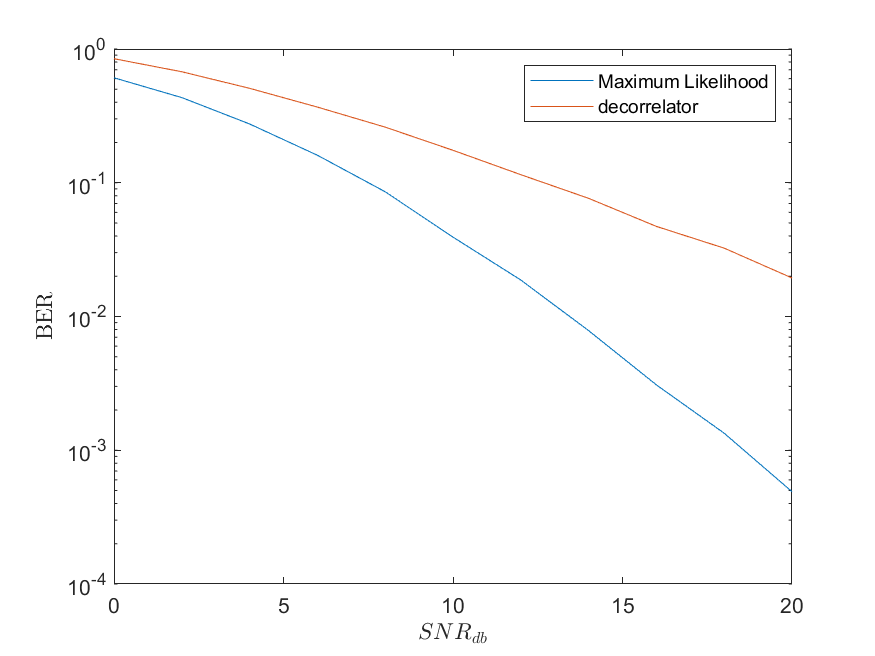
\includegraphics[width=0.5\textwidth]{fig7.png}
					\caption{ML-decorrelator: BER for $SNR_{db}=[0:2:20]$}
				\end{figure}
			
				\begin{figure}[h!]
					\centering
					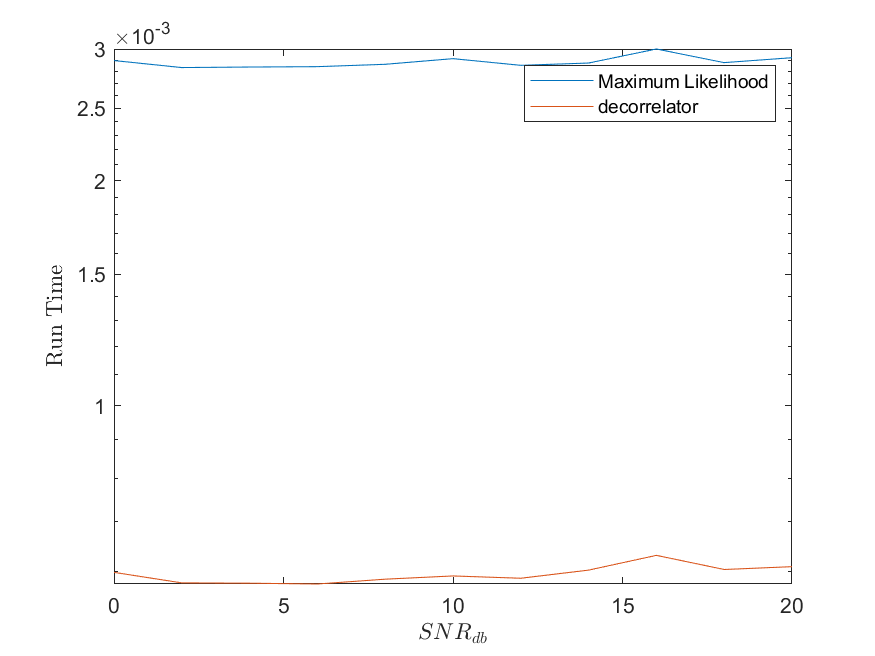
\includegraphics[width=0.5\textwidth]{fig8.png}
					\caption{ML-decorrelator: BER for $SNR_{db}=[0:2:20]$}
				\end{figure}
				As observed from figure 7 the ML method achieves a lower BER than the decorrelator and the difference increases for high snrs. Although from figure 8 the runtime of the decorrelator is lower by an order of magnitude for every snr.
			\end{enumerate}
		\end{enumerate}
	\end{enumerate}
	
\end{document}
